\documentclass{article}
\usepackage{blindtext}
\usepackage{multirow}
\usepackage{amsmath}
\usepackage[utf8]{inputenc}
\usepackage{graphicx}
% bibliography
\usepackage[
    backend=biber,
    style=bwl-FU,
    url=false,
    doi=false,
    eprint=false
]{biblatex}
\addbibresource{Biblio.bib}
\usepackage{threeparttable}
\usepackage{booktabs}
\usepackage{tabularx}
\newcolumntype{L}[1]{>{\raggedright\arraybackslash}p{#1}} % linksbündig mit Breitenangabe
\newcolumntype{C}[1]{>{\centering\arraybackslash}p{#1}} % zentriert mit Breitenangabe
\newcolumntype{R}[1]{>{\raggedleft\arraybackslash}p{#1}} % rechtsbündig mit Breitenangabe
\usepackage{dcolumn}
    \newcolumntype{d}[1]{D{.}{.}{#1}} 

\usepackage[table]{xcolor}
\usepackage{pgfplotstable}


\begin{document}
\title{Some Visualization}
\author{Tobias Klöpper\thanks{Many thanks especially to Marco, his company and the delicious beer he provides}\\
\normalsize University of Zurich
\and Michele Melek Senkal \thanks{Thanks very much to Marco and each member of this group}\\
\normalsize University of Zürich
\and Marco Barcellos \thanks{Many thanks to all the beers that have allowed me to go on}\\
\normalsize University of Minsk
\and David Annoni \thanks{Many thanks to Stack Overflow}\\
\normalsize University of Zurich}
\date{13th of October 2021}
\maketitle
\begin{abstract}
This paper aims to show how to visualize data in a pleasing way so that the audience can better process it
\end{abstract}

\newpage
\section{Table with dcolumn}
The following Table uses dcolumn to visualize the imaginery counsumption of beer and wine per week.
\begin{table}[h]

  \centering
  \begin{tabular}{l*{3}{d{-2}}}

  \toprule
            &  \multicolumn{1}{c}{Czech Republic} & \multicolumn{1}{c}{Germany} & \multicolumn{1}{c}{United States} \\
  \cmidrule(lr){2-2} \cmidrule(lr){3-3} \cmidrule(lr){4-4}
  \midrule  
       Beer &         10.50&   20.89 &  8.54 \\    
       Wine &        5.23 &   10.98   &   19.62 \\
  \bottomrule

  \end{tabular}
\caption{Table using dcolumn}     
\end{table}


\section{Heatmap}
\def\cca#1{\cellcolor{black!#10}\ifnum #1>5\color{white}\fi{#1}}
%For ranges 0-10, multiply by 10 by adding 0 after #1
This table aims to provide insight into average beer sonsumption per day over the period of 2015 to 2020.
\begin{table}[h]
\label{tab1}
\centering
{\setlength\tabcolsep{1.5pt}%
\begin{tabular}{cccccc}
& $CRO$ & $USA$ & $GER$ & $HUN$ & $POL$ \\
$2020$ &  \cca{0} & \cca{0} & \cca{0} & \cca{2} & \cca{0}\\
$2019$ & \cca{0} & \cca{2} & \cca{0} & \cca{2} & \cca{0}\\
$2018$ & \cca{7} & \cca{4} & \cca{3} & \cca{0} & \cca{4}\\
$2017$ & \cca{3} & \cca{0} & \cca{7} &  \cca{4} & \cca{0}\\
$2016$ & \cca{3} & \cca{7} & \cca{7} & \cca{2} &  \cca{4}\\
$2015$ & \cca{2} & \cca{2} & \cca{7} & \cca{2} & \cca{6}\\
\end{tabular}}
\caption{Average Beer Consumption per day}
\end{table}


\section{Line plot color blind-friendly}

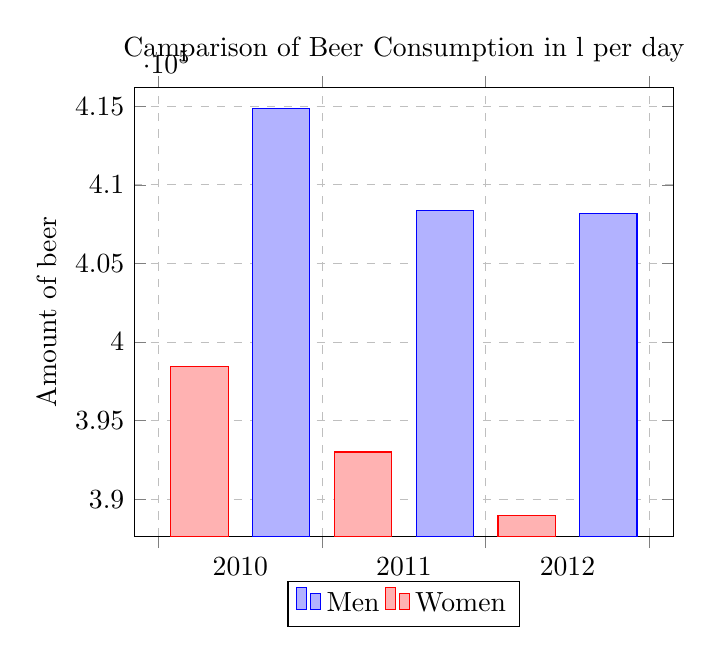
\begin{tikzpicture}
\begin{axis}[
    x tick label style={
        /pgf/number format/1000 sep=},
    title={Camparison of Beer Consumption in l per day},
    ylabel=Amount of beer,
    enlargelimits=0.05,
    legend style={at={(0.5,-0.1)},
    anchor=north,legend columns=-1},
    ybar interval=0.7,
    ymajorgrids=true,
    grid style=dashed,
]
\addplot 
    coordinates {(2012,408184) (2011,408348)
         (2010,414870) (2009,412156)};
\addplot 
    coordinates {(2012,388950) (2011,393007) 
        (2010,398449) (2009,395972)};
\legend{Men,Women}
\end{axis}
\end{tikzpicture}

\section{Why put a grid on plots?}

Sometimes it can be difficult to figure out how high a bar actually is especially if the graph is very large and cotains a lot of different bars. Therefore, the implementation of lines can guide the reader and help asses the real values that are being compared.
\newpage


\end{document}